\documentclass[11pt,a4paper]{article}
\usepackage[T1]{fontenc}
\usepackage[utf8]{inputenc}
\usepackage{lmodern}
\usepackage{amsmath,amssymb,amsthm,mathtools,mathrsfs}
\usepackage{graphicx,float,xcolor,multicol}
\usepackage[shortlabels]{enumitem}
\usepackage[margin=27mm]{geometry}
\usepackage{microtype,needspace,placeins}
\usepackage{tikz,tikz-cd}
\usetikzlibrary{arrows.meta,calc,positioning,patterns,decorations.pathreplacing}
\usepackage[colorlinks=true,linkcolor=teal,urlcolor=teal,citecolor=teal]{hyperref}
\setlength{\parindent}{0pt}
\setlength{\parskip}{.6em}
\setcounter{secnumdepth}{0}
\allowdisplaybreaks
\raggedbottom
\providecommand{\cross}{\times}
\DeclareUnicodeCharacter{2020}{\ensuremath{\dagger}}
\DeclareMathOperator{\supp}{supp}
\DeclareMathOperator*{\esssup}{ess\,sup}
\providecommand{\chapter}{\section}
\newenvironment{tool}[2]{\subsection*{Tool #1 --- #2}}{}
\newcommand{\ToolRef}[1]{Tool #1}
\newcommand{\FigureTag}[2]{\textit{Figure #1}}
\newcommand{\Result}[1]{\subsection*{#1}}
\newcommand{\Application}[1]{\subsubsection*{Application\if\relax\detokenize{#1}\relax\else\space--- #1\fi}}
\newcommand{\ProofHeading}{\par\textit{Proof.}\space}
\newcommand{\ProofOf}[1]{\par\textit{Proof of #1.}\space}
\newcommand{\RemarkHeading}{\par\textbf{Remark.}\space}
\newcommand{\NoteHeading}{\par\textbf{Note.}\space}
\newcommand{\ExerciseHeading}{\par\textbf{Exercise.}\space}

% Rendering support only; mathematical text is in each independent post.
\usepackage{booktabs,array,longtable}
\definecolor{HandoutBlue}{HTML}{2F6690}
\definecolor{HandoutNavy}{HTML}{17365D}
\newtheorem{theorem}{Theorem}
\newtheorem{lemma}[theorem]{Lemma}
\newtheorem{proposition}[theorem]{Proposition}
\newtheorem{corollary}[theorem]{Corollary}
\newtheorem{conjecture}[theorem]{Conjecture}
\newtheorem{definition}{Definition}
\newtheorem{example}{Example}
\newtheorem{namedtoolcounter}{Tool}
\newenvironment{namedtool}[1]{\begin{namedtoolcounter}[#1]}{\end{namedtoolcounter}}
\newtheorem*{claim}{Claim}
\newtheorem*{remark}{Remark}
\newtheorem*{exercise}{Exercise}
\newtheorem*{question}{Question}
\newtheorem*{observation}{Observation}
\newcommand{\SourceChapter}[2]{\section*{#2}}
\newcommand{\Lecture}[2]{\section*{Lecture #1: #2}}
\newcommand{\unclear}[1]{\textit{[unclear: #1]}}
\newcommand{\sourcegap}{\textit{[unfinished in the source]}}
\DeclareMathOperator{\dist}{dist}
\DeclareMathOperator{\id}{id}
\DeclareMathOperator{\Hol}{Hol}
\DeclareMathOperator{\Per}{Per}
\DeclareMathOperator{\Fix}{Fix}
\DeclareMathOperator{\diam}{diam}
\DeclareMathOperator{\Var}{Var}
\DeclareMathOperator{\Leb}{Leb}
\DeclareMathOperator{\Hom}{Hom}
\DeclareMathOperator{\End}{End}
\DeclareMathOperator{\Ann}{Ann}
\DeclareMathOperator{\Spec}{Spec}
\DeclareMathOperator{\Max}{Max}
\DeclareMathOperator{\Ob}{Ob}
\DeclareMathOperator{\Tor}{Tor}
\DeclareMathOperator{\Ass}{Ass}
\DeclareMathOperator{\Mor}{Mor}
\DeclareMathOperator{\Fun}{Fun}
\DeclareMathOperator{\Nat}{Nat}
\DeclareMathOperator{\Cone}{Cone}
\DeclareMathOperator{\MCG}{MCG}
\DeclareMathOperator{\Aut}{Aut}
\DeclareMathOperator{\Deck}{Deck}
\DeclareMathOperator{\SL}{SL}
\DeclareMathOperator{\PSL}{PSL}
\DeclareMathOperator{\Area}{Area}
\DeclareMathOperator{\im}{im}
\DeclareMathOperator{\PSh}{PSh}
\newcommand{\CRing}{\mathsf{CRings}}
\newcommand{\AMod}{A\text{-}\mathsf{Mod}}
\newcommand{\Ab}{\mathsf{Ab}}
\newcommand{\Z}{\mathbb Z}
\newcommand{\Q}{\mathbb Q}
\newcommand{\R}{\mathbb R}
\newcommand{\C}{\mathbb C}
\newcommand{\N}{\mathbb N}
\newcommand{\kk}{\mathbb k}
\renewcommand{\aa}{\mathfrak a}
\newcommand{\bb}{\mathfrak b}
\newcommand{\pp}{\mathfrak p}
\newcommand{\qq}{\mathfrak q}
\newcommand{\mm}{\mathfrak m}
\newcommand{\nn}{\mathfrak n}
\newcommand{\rad}{\mathrm r}
\newcommand{\cat}[1]{\mathsf{#1}}
\setcounter{secnumdepth}{0}
\allowdisplaybreaks

% Notation used only by the newly added notes.
\setlength{\emergencystretch}{2em}
\providecommand{\D}{\mathbb D}
\providecommand{\M}{\mathcal M}
\providecommand{\Chat}{\widehat{\mathbb C}}
\providecommand{\Crit}{\operatorname{Crit}}
\providecommand{\Int}{\operatorname{Int}}
\providecommand{\Ext}{\operatorname{Ext}}

\graphicspath{{figures/quadratic-family/}}
\begin{document}
\section*{The Quadratic Family}
% BLOG-CONTENT-BEGIN
% Source page 1
\section{Normalization and the Mandelbrot set}
Start with $f(z)=az^2+bz+c$. Conjugating by a dilation gives
\[
\lambda^{-1}f(\lambda z)=z^2+\alpha z+\beta,
\qquad \lambda=\frac1a.
\]
We then conjugate by a translation:
\[
\begin{aligned}
(z-d)\circ(z^2+\alpha z+\beta)\circ(z+d)
 &=(z+d)^2+\alpha(z+d)+\beta-d\\
 &=z^2+(2d+\alpha)z+d^2-d+\beta.
\end{aligned}
\]
Taking $d=-\alpha/2$, the critical point, gives the normal form $z^2+c$, denoted by $P_c$.

Suppose that an affine map $\varphi(z)=\lambda z+d$ satisfies $\varphi^{-1}\circ P_c\circ\varphi=P_{c'}$. Comparing the quadratic, linear, and constant coefficients gives $\lambda=1$, $d=0$, and $c=c'$. Thus every affine-conjugacy class of quadratic polynomials has a unique representative $P_c$. Thus
\[
\Moduli(\text{quadratic polynomials})\cong\C.
\]

\setcounter{definition}{0}\begin{definition}[Mandelbrot set]
The \emph{Mandelbrot set} is
\[
\M:=\{c\in\C\mid (P_c^{\circ n}(0))_{n\ge0}\text{ is bounded}\}.
\]
\end{definition}

\setcounter{theorem}{1}\begin{corollary}[Connected Julia sets]
\[
\M=\{c\mid K(P_c)\text{ is connected}\}
    =\{c\mid J(P_c)\text{ is connected}\}.
\]
\end{corollary}

% Source page 4
\subsection{Escape bounds and the real slice}
\setcounter{theorem}{2}\begin{theorem}[Basic properties of the Mandelbrot set]\label{thm:basic-properties}
\begin{enumerate}[label=(\roman*)]
\setcounter{enumi}{0}\item $\M\subseteq\{c\mid |c|\le2\}$, $\M$ is compact and connected, and $\Chat\setminus\M$ is simply connected.
\setcounter{enumi}{1}\item $\M\cap\mathbb R=[-2,1/4]$.
\setcounter{enumi}{2}\item $|P_c^{\circ n}(0)|\le2$ for all $n\ge1$ if and only if $c\in\M$.
\end{enumerate}
\end{theorem}

\begin{proof}
\textit{(i)} If $|c|>2$, put $z_n=P_c^{\circ n}(0)$. Then $|z_1|=|c|$, and whenever $|z_n|\ge |c|$,
\[
|z_{n+1}|\ge |z_n|^2-|c|
\ge |z_n|(|z_n|-1)
\ge (|c|-1)|z_n|.
\]
Thus $|z_n|\to\infty$ and $c\notin\M$, proving the asserted bound.

\textit{(iii)} Suppose $|P_c^{\circ m}(0)|=2+\delta>2$ for some $m\ge1$. If $|c|=|P_c(0)|>2$, then $c\notin\M$. If $|c|\le2$, then
\[
|P_c^{\circ(m+1)}(0)|\ge(2+\delta)^2-2\ge2+4\delta.
\]
By induction, $|P_c^{\circ(m+k)}(0)|\ge2+4^k\delta\to\infty$, so again $c\notin\M$. If $c_m\to c$ with $c_m\in\M$, then $|P_c^{\circ n}(0)|\le2$ for every $n$; hence $\M$ is closed.

The connectedness of $\M$ and the simple connectedness of $\Chat\setminus\M$ will follow from the uniformisation of $\Chat\setminus\M$ below.

\textit{(ii)} For $c\in\mathbb R$, the polynomial $P_c(x)-x$ has no real roots if $c>1/4$, one real root if $c=1/4$, and two real roots if $c<1/4$. If $c>1/4$, then $P_c^{\circ n}(0)\to\infty$; otherwise the orbit would accumulate at an $x\in\mathbb R$ with $P_c(x)=x$.

If $c\le1/4$, let $a=(1+\sqrt{1-4c})/2$ be the larger of the two roots of $P_c(x)-x$. If also $c\ge-2$, then $a\ge|c|=|P_c(0)|$.

% Source page 5
For $|x|\le a$, we have
\[
-a\le c\le x^2+c\le a^2+c=a.
\]
Therefore $|P_c(x)|\le a$, and induction shows that $|P_c^{\circ n}(0)|\le a$ for every $n$. The sequence $\{P_c^{\circ n}(0)\}_n$ is bounded, and $\M\cap\mathbb R=[-2,1/4]$.
\end{proof}

\Needspace{10\baselineskip}
\subsection{Attracting cycles and stability}
\setcounter{theorem}{3}\begin{theorem}[Continuation of attracting cycles]\label{thm:attracting-continuation}
Let $a\in\Int(\M)$, and suppose $P_a$ has an attracting cycle of length $m$. Let $W$ be the component of $\Int(\M)$ containing $a$. Then, for every $c\in W$, $P_c$ has an attracting cycle $\{z_1(c),\ldots,z_m(c)\}$ of length $m$, and $c\mapsto z_i(c)$ is holomorphic for every $1\le i\le m$.
\end{theorem}

\setcounter{theorem}{4}\begin{theorem}[Density of the interior]\label{thm:interior-dense}
$\Int(\M)$ is dense in $\M$.
\end{theorem}
\begin{proof}
Let $U$ be a disk that meets $\partial\M$, with $0\notin U$.
\begin{figure}[H]
\centering
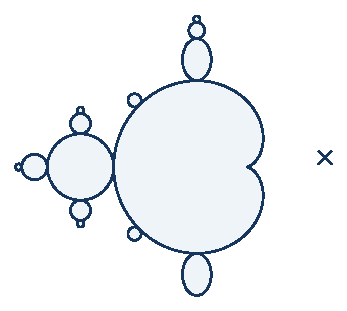
\includegraphics[width=7.5cm,height=4.7cm,keepaspectratio]{qf-fig-01.pdf}
\FigureTag{QF1}{fig:qf-01}
\end{figure}
Suppose $U$ contains no parameter for which $0$ is periodic under $P_c$. Choose a branch of $\sqrt{-c}$ on $U$. Then
\[
P_c^{\circ n}(0)\ne0,\ \pm\sqrt{-c},
\]
since either of the latter two equalities would give $P_c^{\circ(n+1)}(0)=0$. Consequently,
\[
\left\{\frac{P_c^{\circ n}(0)}{\sqrt{-c}}\right\}_n
\]
omits $0,1,-1$ and is normal on $U$. Choose a convergent subsequence. On the nonempty open set $U\cap\Ext(\M)$ it tends to $\infty$, so its limit is identically $\infty$. But $U$ also contains a parameter of $\M$, at which the critical orbit, and hence this subsequence, is bounded. This contradiction proves that $U$ contains a parameter for which $0$ is periodic.
\end{proof}

\setcounter{theorem}{5}\begin{corollary}[$J$-stability]
\[
\{c\mid P_c\text{ is }J\text{-stable}\}=\C\setminus\partial\M.
\]
\end{corollary}
% Source page 7
\Needspace{13\baselineskip}
\section{Components and invariant line fields}
\subsection{Non-hyperbolic components}
\setcounter{theorem}{6}\begin{theorem}[Invariant line fields]\label{thm:line-fields}
If $c\in\Int(\M)$, then the component of $\Int(\M)$ containing $c$ is non-hyperbolic if and only if $J(P_c)$ has positive measure and carries an invariant line field.
\end{theorem}

\begin{figure}[H]
\centering
\begin{minipage}[c]{.26\linewidth}
\centering

\includegraphics[width=\linewidth,height=2cm,keepaspectratio]{qf-fig-02.pdf}
\FigureTag{QF2}{fig:qf-02}
\end{minipage}\hfill
\begin{minipage}[c]{.68\linewidth}
\centering
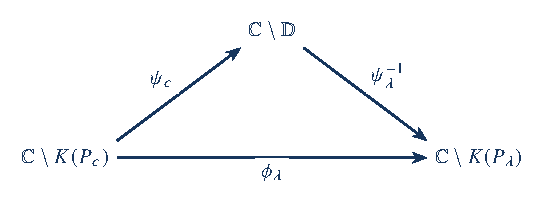
\includegraphics[width=\linewidth,height=4.8cm,keepaspectratio]{qf-fig-03.pdf}
\FigureTag{QF3}{fig:qf-03}
\end{minipage}
\end{figure}

\begin{figure}[H]
\centering
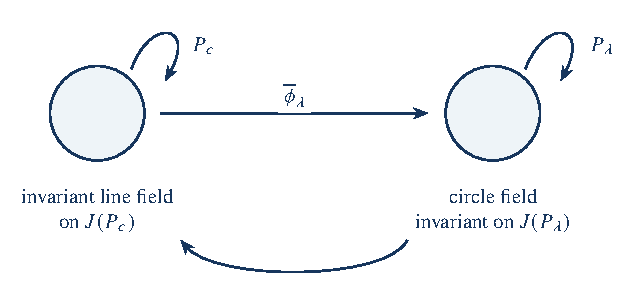
\includegraphics[width=12cm,height=5.1cm,keepaspectratio]{qf-fig-04.pdf}
\FigureTag{QF4}{fig:qf-04}
\end{figure}

% Source page 9
% Source page 10
\section{Quasicircles and uniformisation}
\subsection{The principal hyperbolic component}
\setcounter{theorem}{7}\begin{theorem}[Quasicircle Julia sets]
If $c$ is in the principal hyperbolic component, then $J(P_c)$ is a quasicircle.
\end{theorem}

\begin{figure}[H]
\centering
\begin{minipage}[c]{.45\linewidth}
\centering
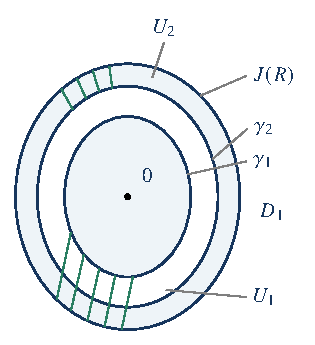
\includegraphics[width=\linewidth,height=6.4cm,keepaspectratio]{qf-fig-05.pdf}
\FigureTag{QF5}{fig:qf-05}
\end{minipage}\hfill
\begin{minipage}[c]{.49\linewidth}
\centering
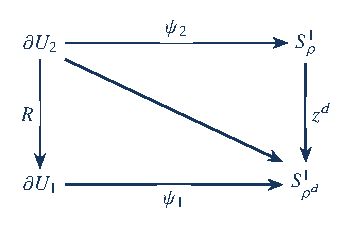
\includegraphics[width=\linewidth,height=4.7cm,keepaspectratio]{qf-fig-06.pdf}
\FigureTag{QF6}{fig:qf-06}
\end{minipage}
\end{figure}

\subsection{Uniformisation of the complement of the Mandelbrot set}
Recall that, if $c\in\M^c$, then $A_c(\infty)$ is the only Fatou component, and the Julia set is totally disconnected.

% Source page 12
\begin{figure}[H]
\centering
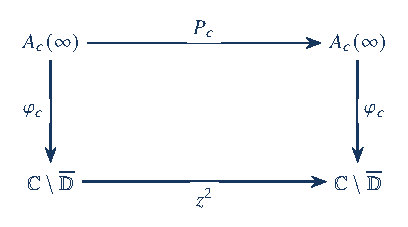
\includegraphics[width=8.5cm,height=4.5cm,keepaspectratio]{qf-fig-07.pdf}
\FigureTag{QF7}{fig:qf-07}
\end{figure}

The B\"ottcher map satisfies
\[
\varphi_c(P_c(z))=\varphi_c(z)^2,
\qquad
\varphi_c(z)=\lim_{n\to\infty}[P_c^n(z)]^{2^{-n}}.
\]
Moreover,
\[
\begin{aligned}
\varphi_c(z)
 &=z\prod_{n=1}^{\infty}
 \left(\frac{P_c^n(z)}{P_c^{n-1}(z)^2}\right)^{2^{-n}}\\
 &=z\prod_{n=0}^{\infty}
 \left(1+\frac{c}{P_c^n(z)^2}\right)^{2^{-(n+1)}}.
\end{aligned}
\]
Hence, if defined,
\[
\varphi_c(c)=c\prod_{n=0}^{\infty}
 \left(1+\frac{c}{P_c^n(c)^2}\right)^{2^{-(n+1)}},
\]
which has a simple pole at $\infty$.

Using $\varphi_c(P_c(z))=\varphi_c(z)^2$, we can extend $\varphi_c$ conformally until we hit a critical point of $P_c$, namely $0$. Set $G_c(z)=\log|\varphi_c(z)|$. Then
\begin{equation}\label{eq:green-functional}
G_c(P_c(z))=2G_c(z).
\tag{$\star$}
\end{equation}
The Green function $G_c$ extends to all of $A_c(\infty)$.

For $G_c(z)>G_c(0)$, the map $\varphi_c(z)$ is analytic and maps that set conformally to $\{\zeta\mid |\zeta|>e^{G_c(0)}\}$. Also,
\[
K(P_c)=\bigcap_{n=1}^{\infty}
P_c^{-n}\bigl(\{z\mid G_c(z)\le G_c(0)\}\bigr).
\]
By \eqref{eq:green-functional}, as $z\to\partial A_c(\infty)$, that is, $J(P_c)$, we have $G_c(z)\to0$. Extend $G_c$ to the whole plane by defining it to be zero elsewhere.

% Source page 13
The function $G_c(z)$ is jointly continuous in $c$ and $z$. Notice that
\[
P_c(0)=c\quad\Longrightarrow\quad G_c(c)=2G_c(0)>G_c(0).
\]
Thus $\varphi_c(c)$ is well-defined and analytic in $c$. As $c\to\M$, say $c_n\to c_0\in\M$, we have $G_{c_n}(z)\to G_{c_0}(z)$ locally uniformly in $\C$, so
\[
G_{c_n}(c_n)\longrightarrow G_{c_0}(c_0)=0
\qquad\bigl(\text{because }c_0\in K(P_{c_0})\bigr).
\]
Consequently, $|\varphi_c(c)|\to1$ as $c\to\M$. We therefore have an analytic map, with a simple pole at $\infty$,
\[
\Chat\setminus\M\longrightarrow\Chat\setminus\overline\D,
\qquad c\longmapsto\varphi_c(c).
\]
This map is a conformal isomorphism from $\Chat\setminus\M$ onto $\Chat\setminus\overline\D$.
% BLOG-CONTENT-END
\end{document}
